This section shows the results obtained with the simulation of the TRITIUM-IFIC 2 prototype, which was used for two different objectives. On the one hand, these simulations were carried out to find the Low Detection Limit, LDL, of this prototype for tritiated water activity, which is an important parameter to know the limitation of the prototype. On the other hand, these simulations serve to study the activity resolution of the prototype and  how it can be improved through various parameters such as the increasement of the integration counting count time of the measurement or the number of prototypes read in parallel.

The detection of a tritium event by the TRITIUM-IFIC 2 prototype is shown in Figure \ref{fig:TritiumEventDetectedInSimulatedPrototype}, in which, the path followed by the photons created in scintillating fibers are represented by green lines which end in red dots when it is absorbed in the fiber or the water and blue dots when it is absorbed in the PMTs (detected). The fiber that has detected the tritium electron is clearly identfied and the photons out of this are those that has not been collected due to the critical angle. Blue dots are obtained in both PMTs for this event, indicating that this is detected on time coincidence.

\begin{figure}[hbtp]
\centering
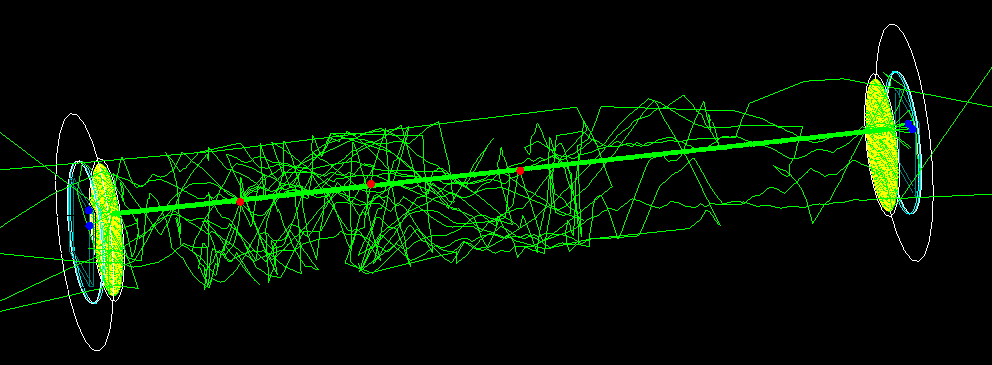
\includegraphics[scale=0.35]{Figures/8SimulationsResults/82TRITIUMMonitor/821TRITIUMIFIC2/EventDetectedInTRITIUMIFIC2.png}
\caption{Tritium electron detected in the simulated TRITIUM-IFIC 2 prototype. The path of the optical photons is represented by green lines and the position in which it is absorbed is represented by red and blue dots (absorbed in water or PMT, respectively).\label{fig:TritiumEventDetectedInSimulatedPrototype}}
\end{figure}

Several variables were used as tests in each simulation to verify the different steps of the simulation such as the production of tritium events, the energy deposition in scintillating fibers and their subsequent photon emission, spatial distribution of generated events, detected events, etc. %Some of these variables are detailed in the appendix \ref{App:TestVariablesSimulations}.

The distribution of the number of photons detected by both PMTs per tritium event was obtained for the simulated TRITIUM-IFIC 2 prototype, shown in Figure \ref{fig:SimulatedPhotonsDetected}.

\begin{figure}[hbtp]
\centering
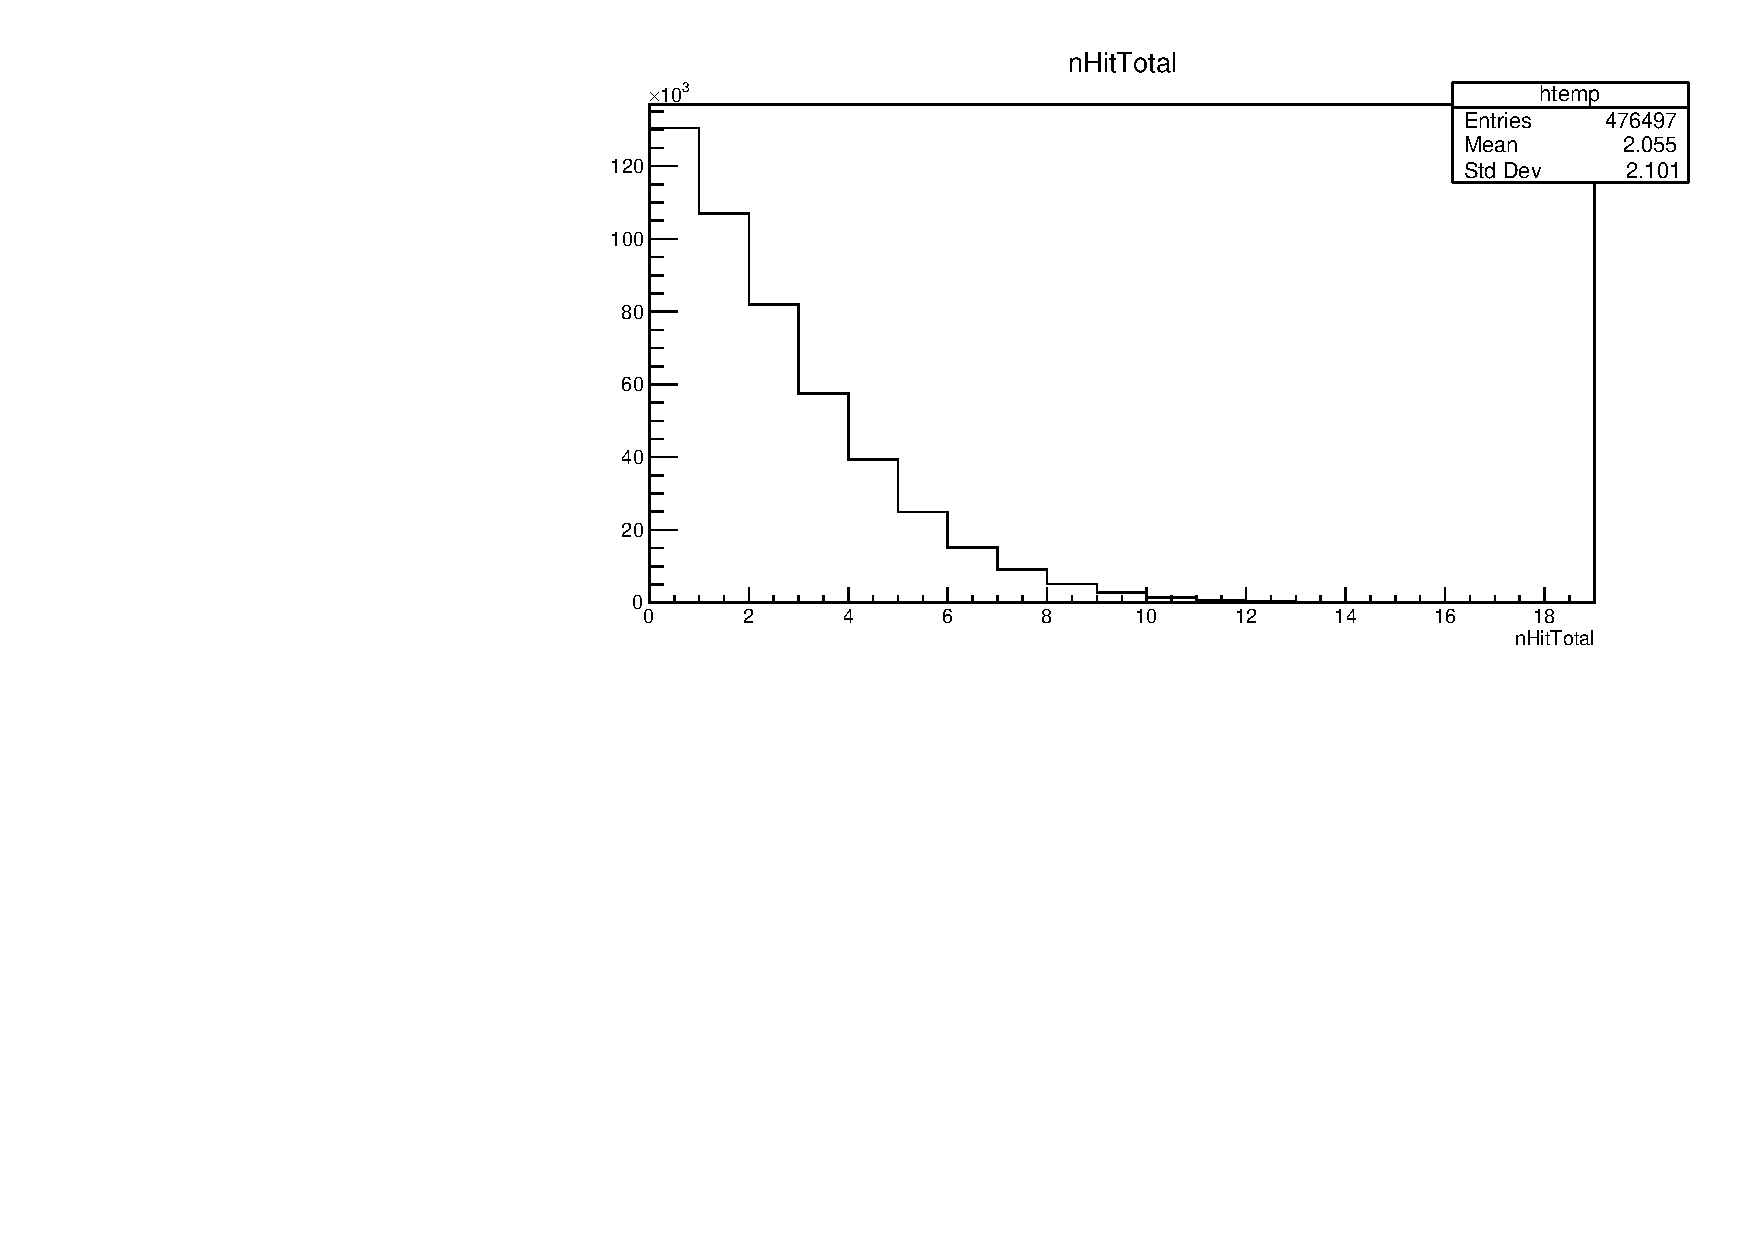
\includegraphics[scale=0.65]{Figures/8SimulationsResults/82TRITIUMMonitor/821TRITIUMIFIC2/PhotonsDetected_simulation.pdf}
\caption{Photons detected by both PMTs per tritium event in the simulated TRITIUM-IFIC 2 prototype.\label{fig:SimulatedPhotonsDetected}}
\end{figure}

A maximum of $17$ photons is obtained for the TRITIUM-IFIC 2 prototype simulations, which are in agreement with the maximum of $15$ photons experimentaly measured by the experimental experience, Figure \ref{subfig:TritiumSignalTRITIUMIFIC2}. This confirms that the value used in the simulations for the Birks coefficient, $k_B=0.136~\mm/\MeV$, is adequate. The experimentally obtained distribution are a bit small between $3$ and $8$ photons, probably due to imperfections of the prototype which are impossible to simulate.

Various activities were simulated from $100~\becquerel/\liter$ to $5~\kilo\becquerel/\liter$ for three months of simulated data taking and an integration counting time of $10~\min$ was used.

The measurements obtianed are presented in Figure \ref{subfig:RawData1Det10Min250BqL} as a function of time, which are histogramed in Figure \ref{subfig:Dist1Det10Min250BqL}. 

\begin{figure}
\centering
    \begin{subfigure}[b]{0.7\textwidth}
    \centering
    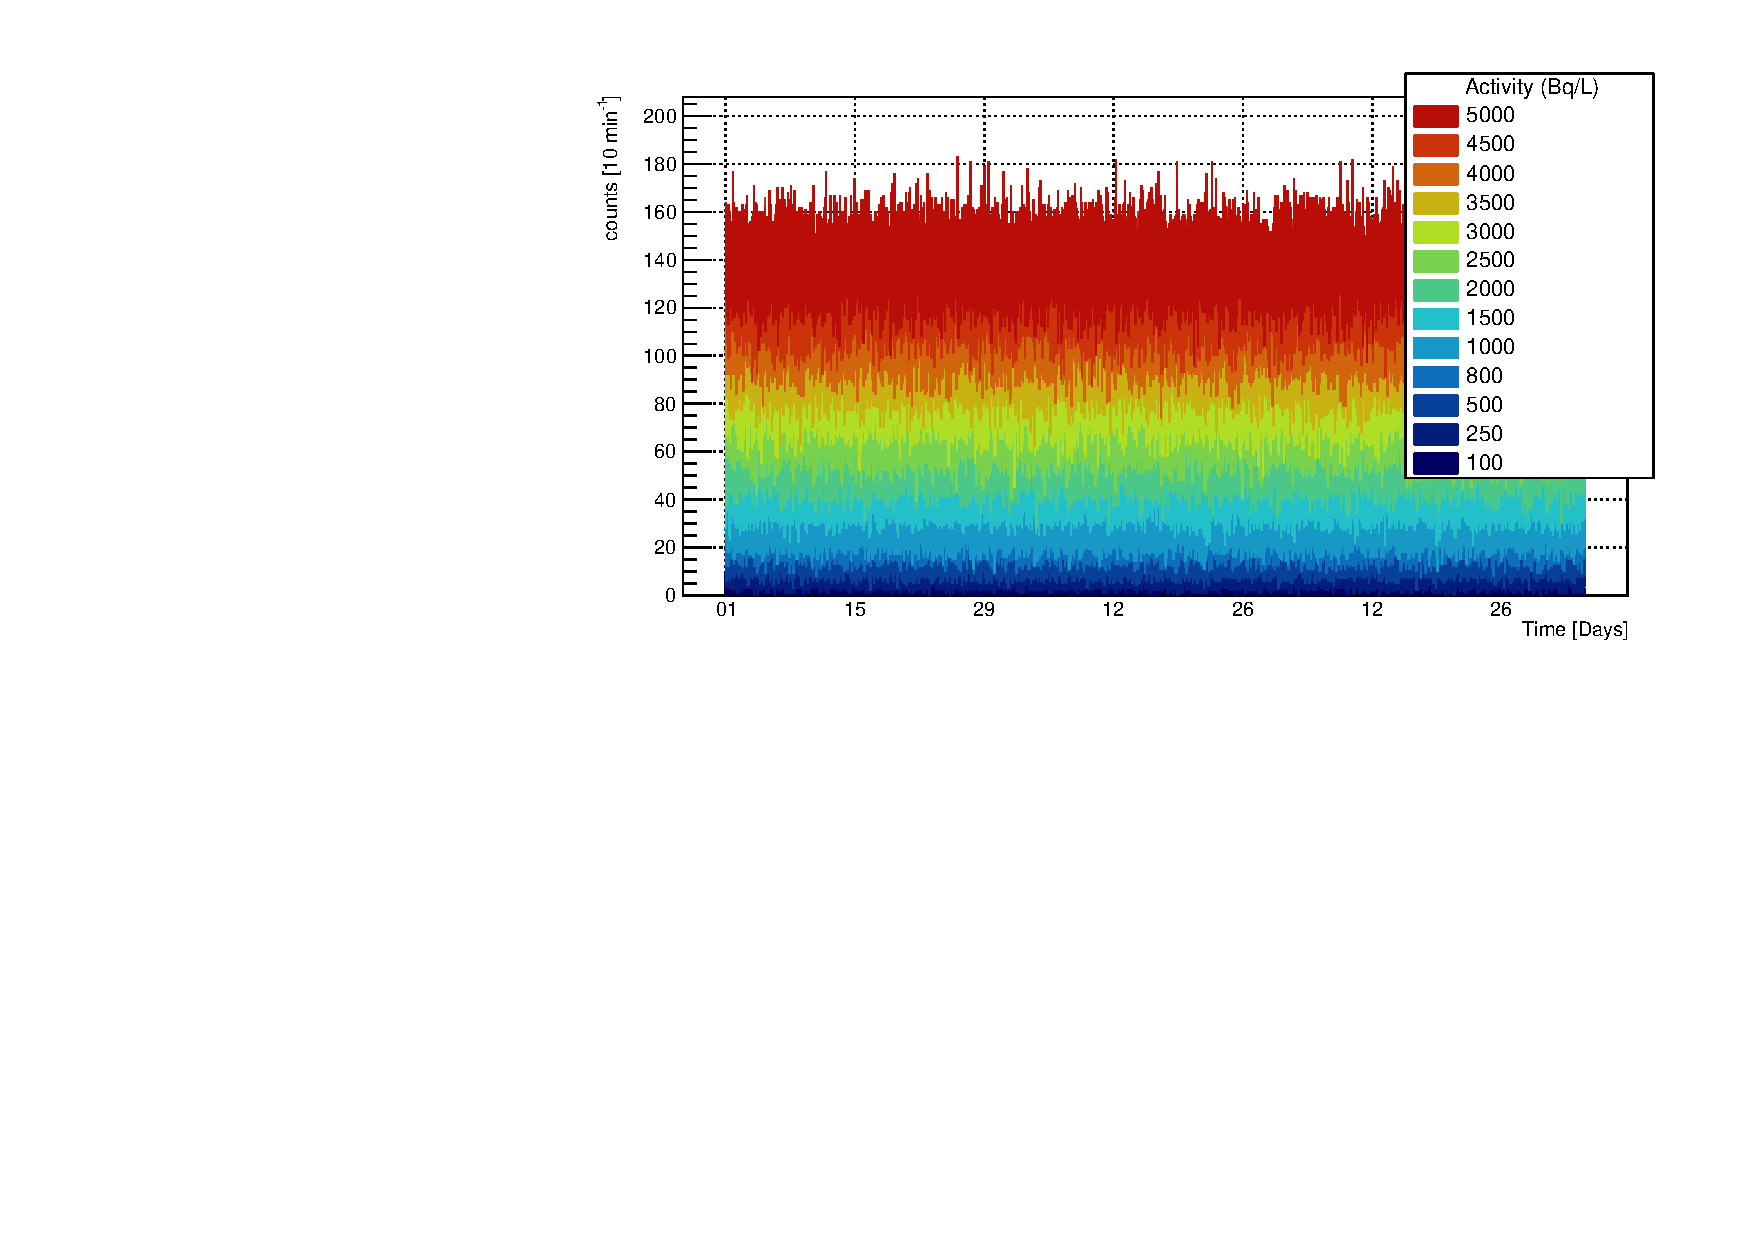
\includegraphics[width=\textwidth]{8SimulationsResults/82TRITIUMMonitor/821TRITIUMIFIC2/RawData_1Det_10min_250BqL.pdf}  
    \caption{\label{subfig:RawData1Det10Min250BqL}}
    \end{subfigure}
    \hfill
    \begin{subfigure}[b]{0.7\textwidth}
    \centering
    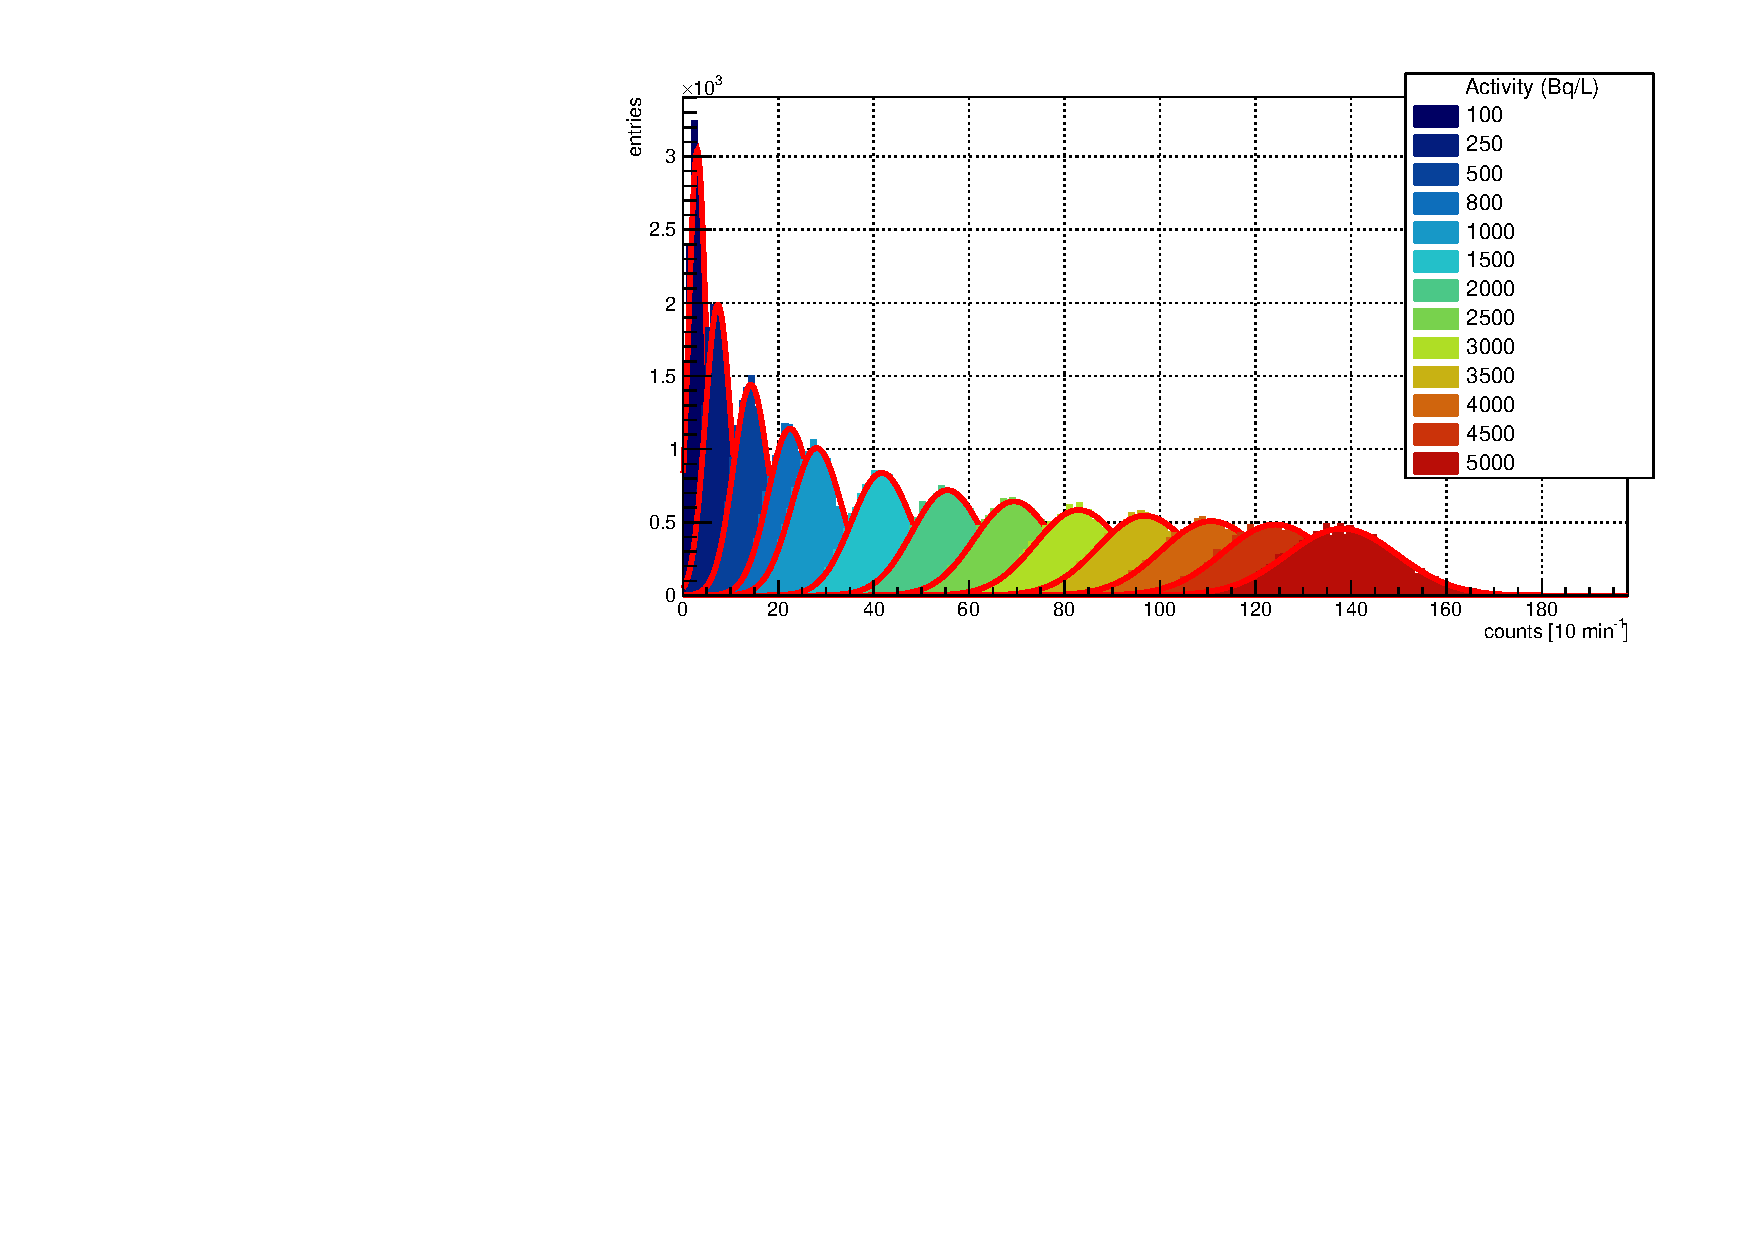
\includegraphics[width=\textwidth]{8SimulationsResults/82TRITIUMMonitor/821TRITIUMIFIC2/Dist_1Det_10min_250BqL_and_Gaus.pdf}  
    \caption{\label{subfig:Dist1Det10Min250BqL}}
    \end{subfigure}
 \caption{Tritium counts detected with a simulated TRITIUM-IFIC 2 prototype using a integration counting time of $10~\min$ a) as a function of the time b) distribution of them.}
 \label{fig:1Det10Min250BqL}
\end{figure}

Difference of $250~\becquerel/\liter$ is not distinguished due to the overlapping of sevarial distributions. To reduce the width of the distribution obtianed for each activity, the stadistics must be increased, which can be done in two different ways, increasing the integration counting time or increasing the number of prototype read in parallel.

To check the effect due to an increasement of the integration counting time similar distributions are obtained for three increasing integration counting times ($10~\min$, $30~\min$ and $60~\min$), which are shown in Figure \ref{fig:1Det250BqLseveralTimes}. 

\begin{figure}
\centering
    \begin{subfigure}[b]{0.6\textwidth}
    \centering
    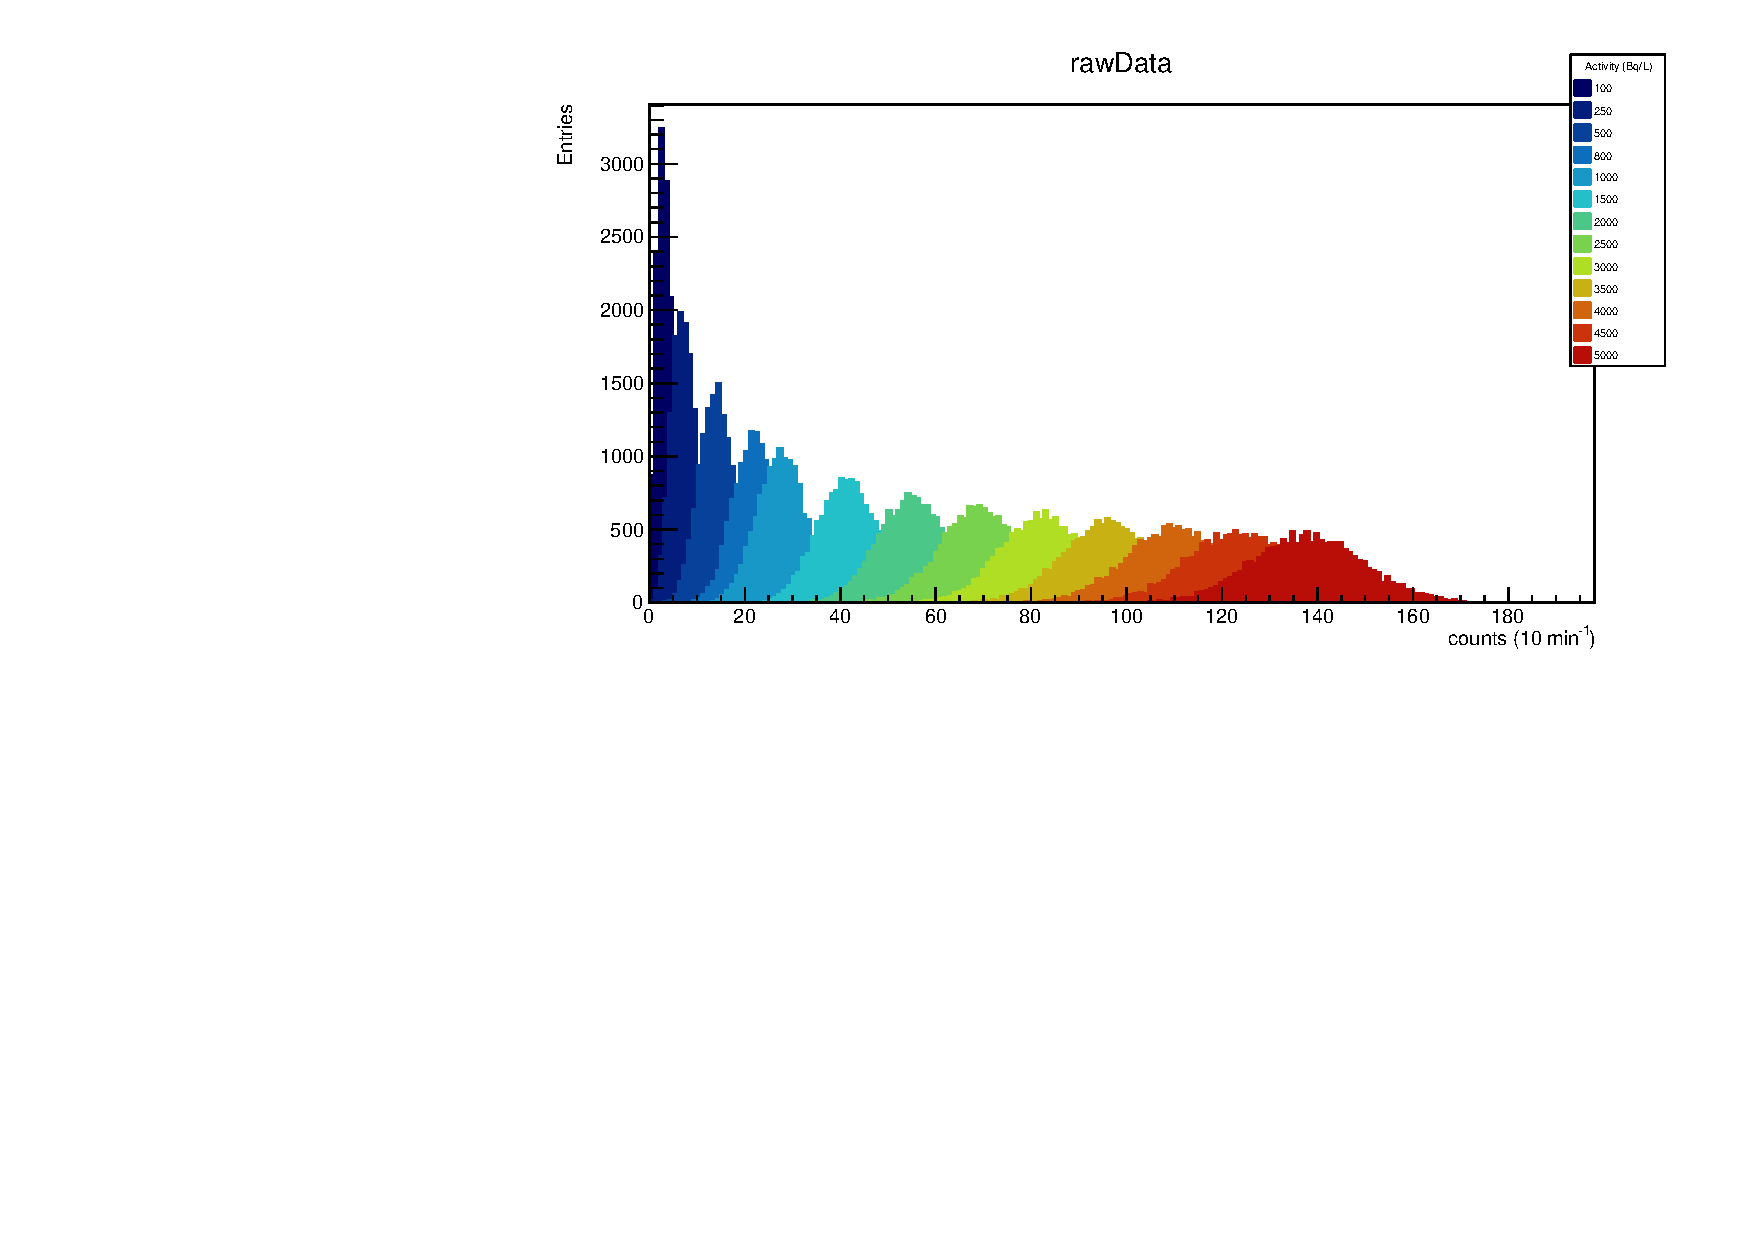
\includegraphics[width=\textwidth]{8SimulationsResults/82TRITIUMMonitor/821TRITIUMIFIC2/Dist_1Det_10min_250BqL.pdf}  
    \caption{\label{subfig:1Det10min250BqLST}}
    \end{subfigure}
    \hfill
    \begin{subfigure}[b]{0.6\textwidth}
    \centering
    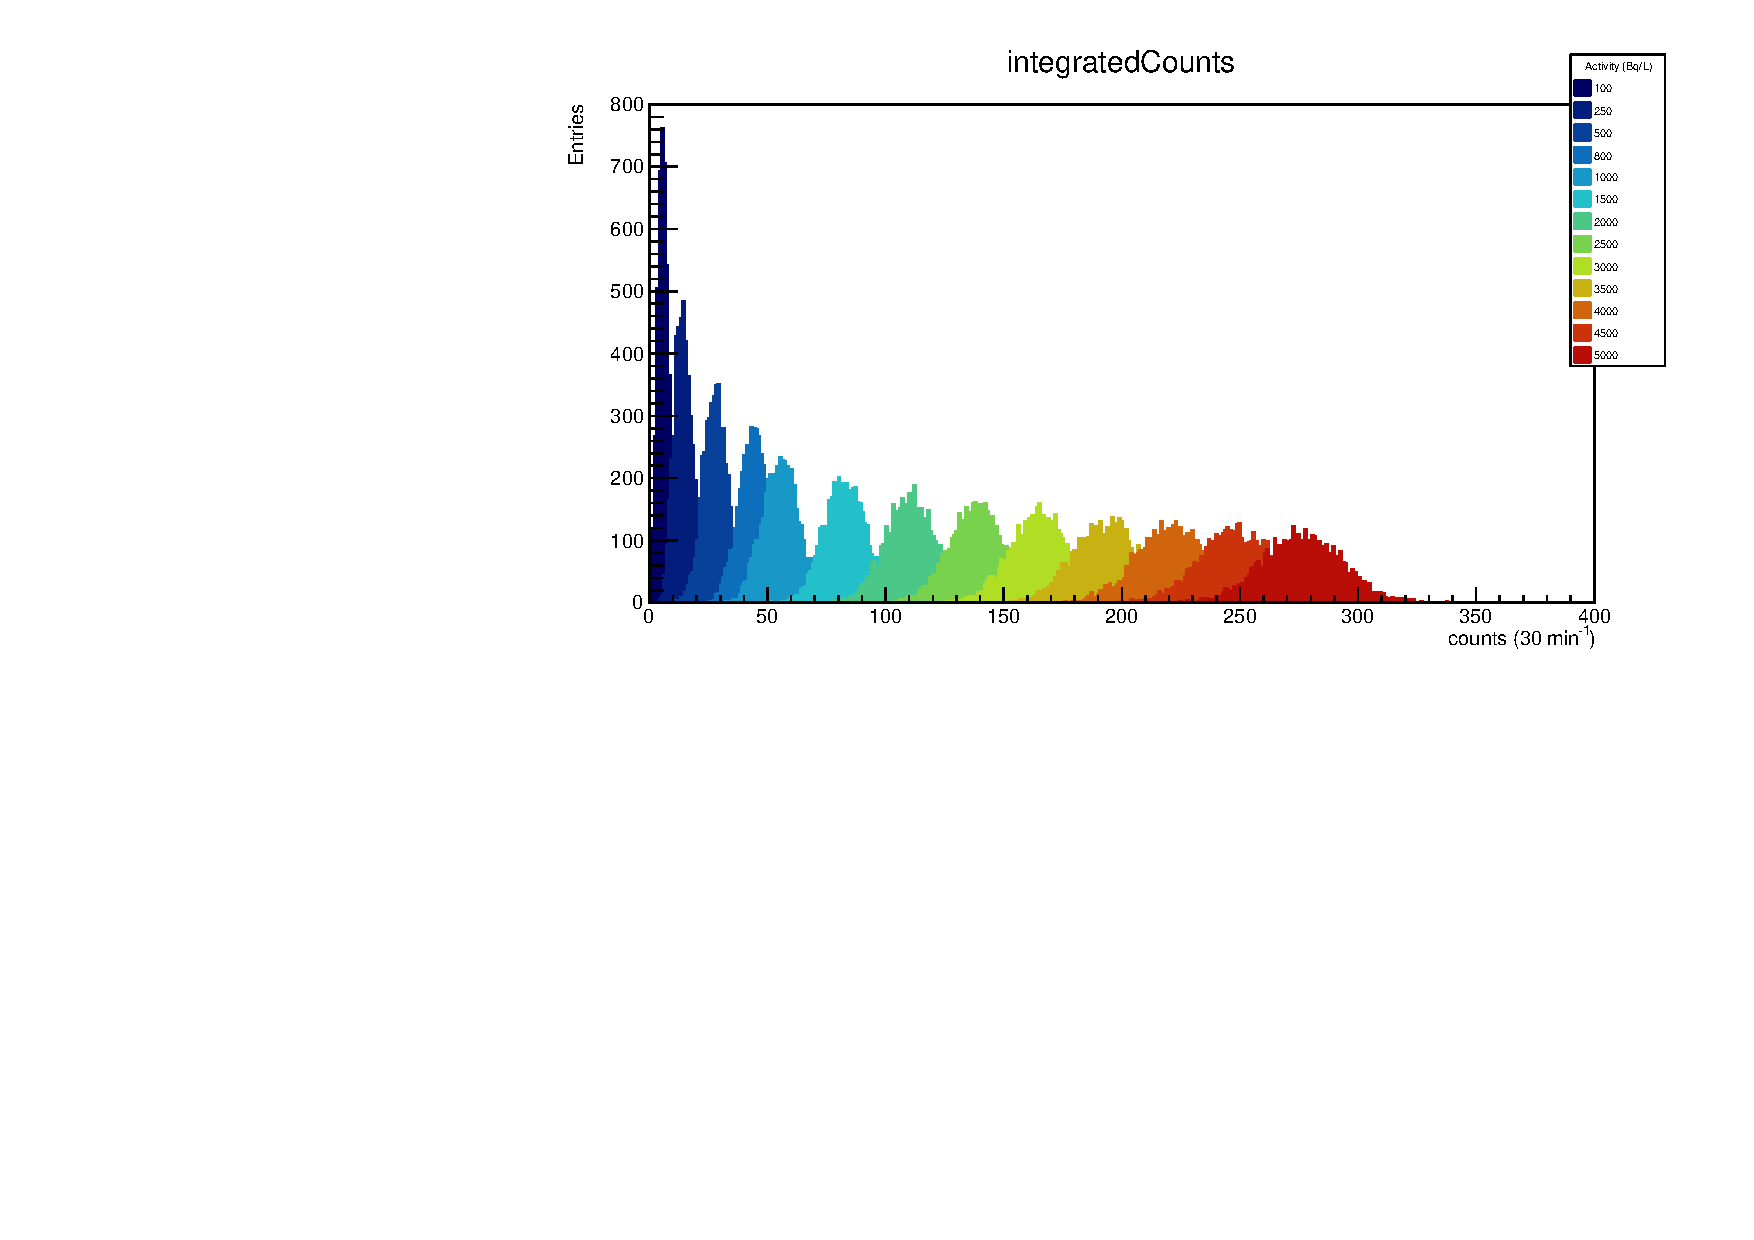
\includegraphics[width=\textwidth]{8SimulationsResults/82TRITIUMMonitor/821TRITIUMIFIC2/Dist_1Det_30min_250BqL.pdf}  
    \caption{\label{subfig:1Det30min250BqLST}}
    \end{subfigure}
    \hfill
    \begin{subfigure}[b]{0.6\textwidth}
    \centering
    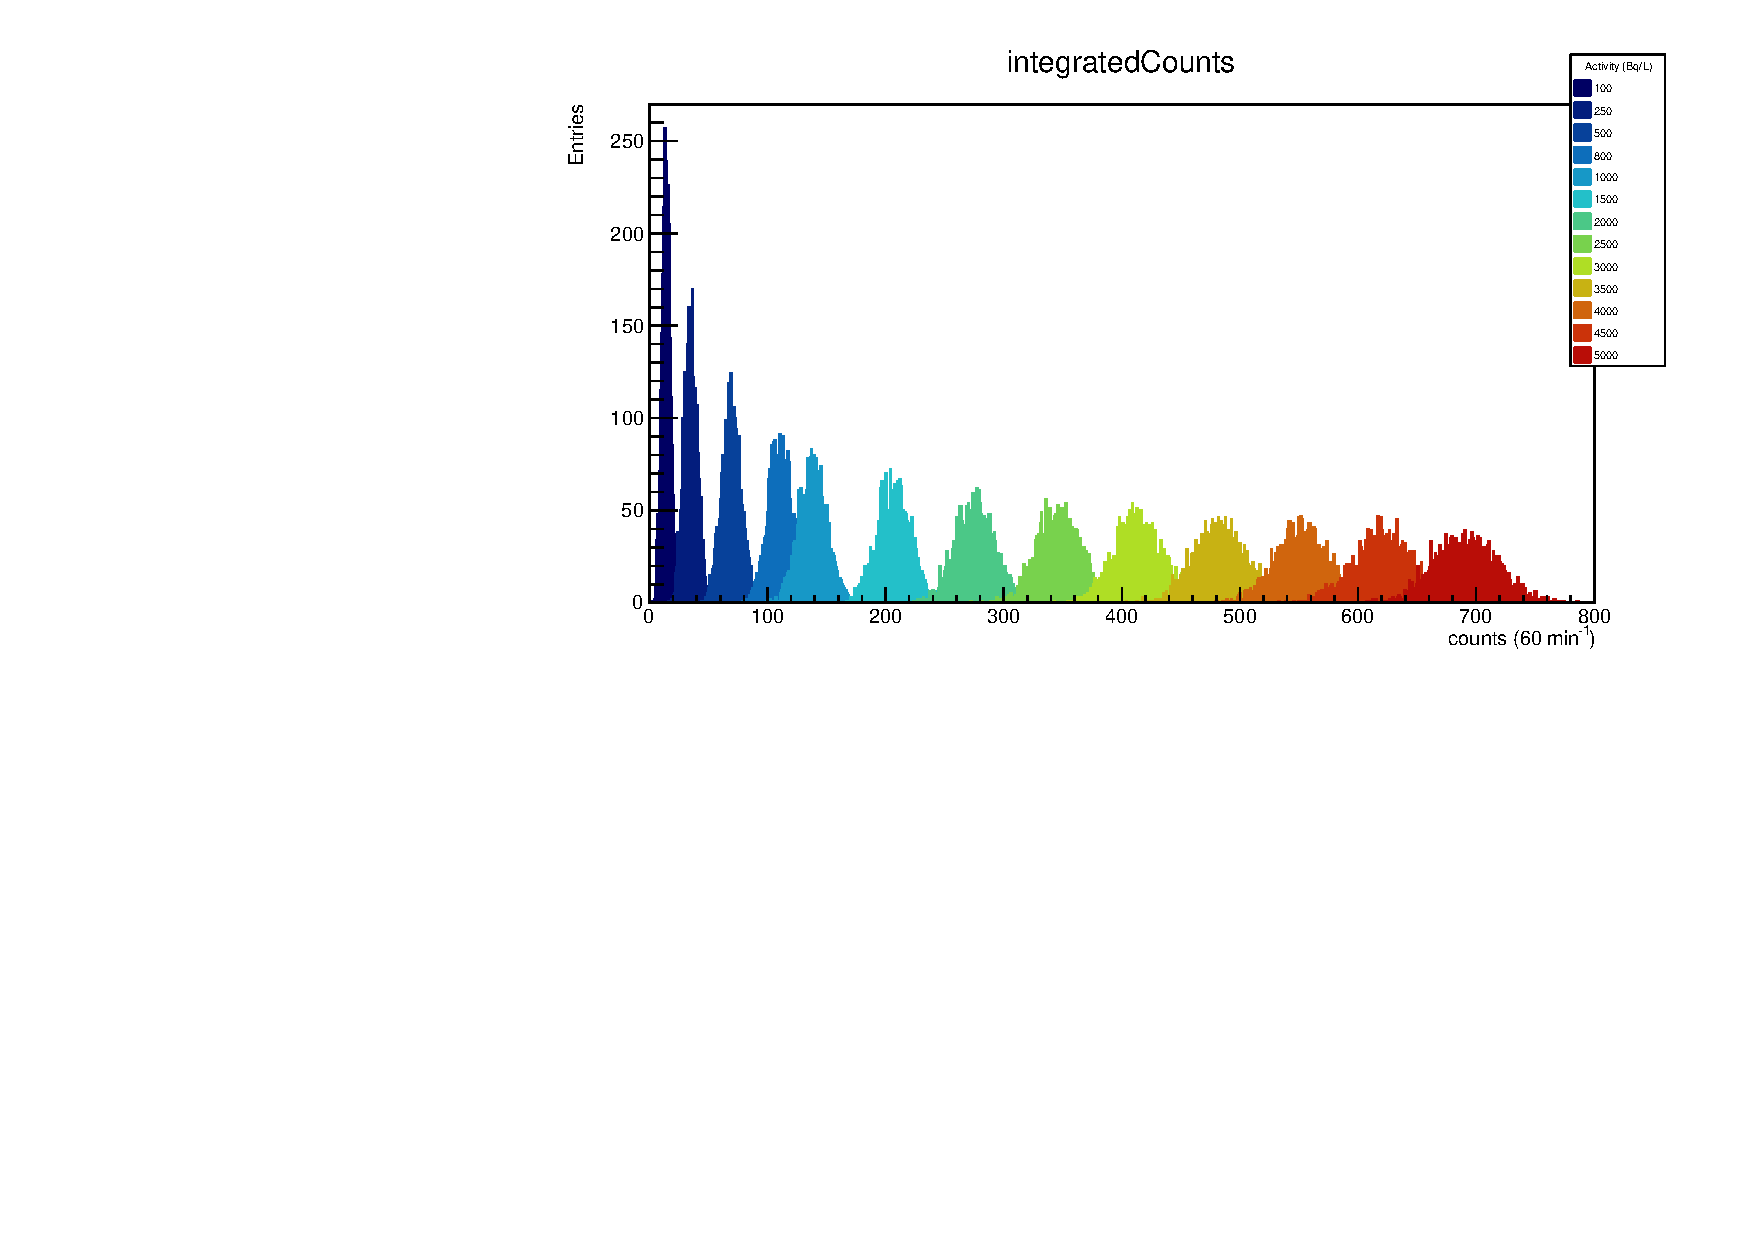
\includegraphics[width=\textwidth]{8SimulationsResults/82TRITIUMMonitor/821TRITIUMIFIC2/Dist_1Det_60min_250BqL.pdf}  
    \caption{\label{subfig:1Det60min250BqLST}}
    \end{subfigure}
 \caption{The distribution of the tritium counts detected with a simulated TRITIUM-IFIC 2 prototype for three different integration counting time, a)$10~\min$ b) $30~\min$ and c) $60~\min$.}
 \label{fig:1Det250BqLseveralTimes}
\end{figure}

The effect of increasing the integration counting time is clearly visible in this figure, reducing the relative distribution width and improving the activity resolution of the TRITIUM monitor. Difference as low as $250~\becquerel/\liter$ are clearly distiguised using only one detector and an integration counting time of $60~\min$, which we can still consider a quasi-real time measurement. Similarly, this distributions are shown in Figure \ref{fig:SeveralDet250BqL10min} for $10~\min$ of integration counting time, in which three increasing number of prototypes were read in parallel (1, 5 and 10).

\begin{figure}
\centering
    \begin{subfigure}[b]{0.6\textwidth}
    \centering
    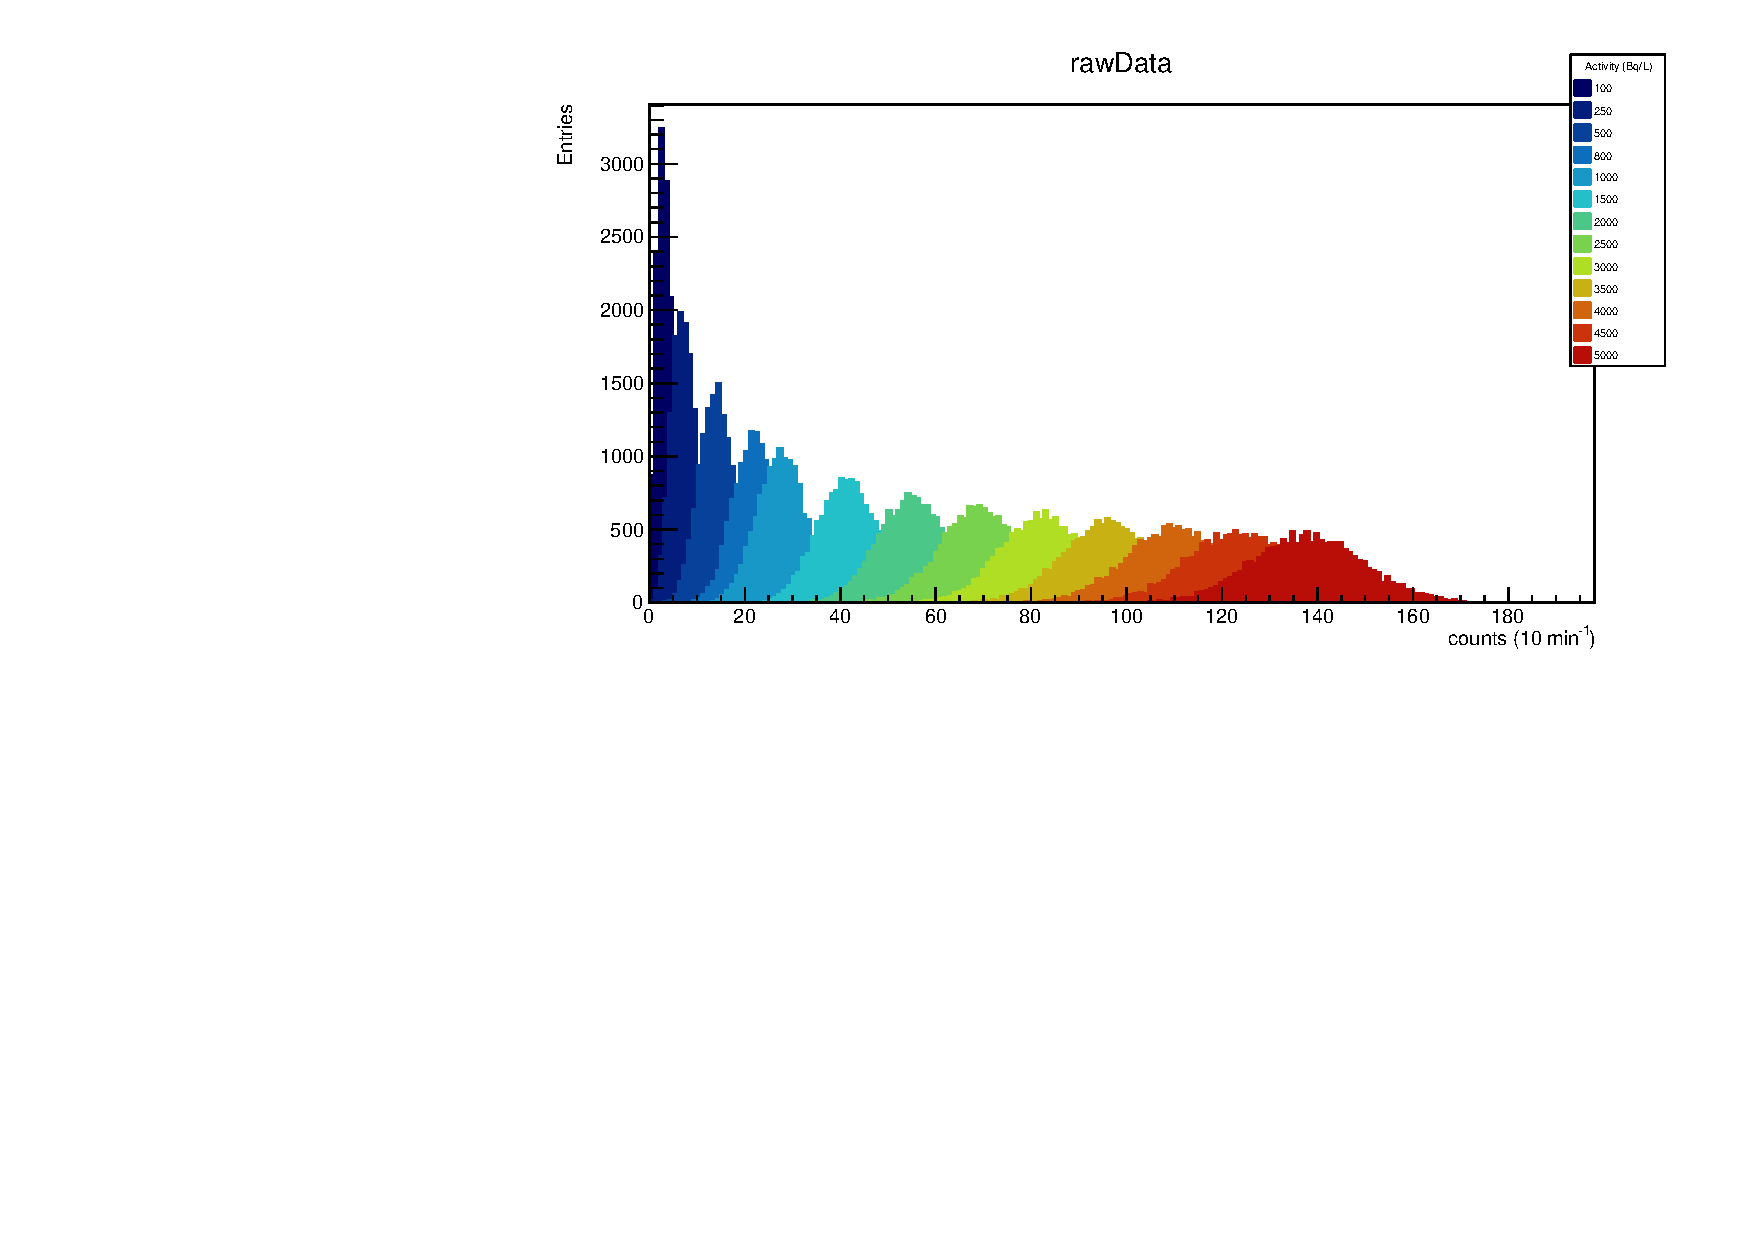
\includegraphics[width=\textwidth]{8SimulationsResults/82TRITIUMMonitor/821TRITIUMIFIC2/Dist_1Det_10min_250BqL.pdf}  
    \caption{\label{subfig:1Det10min250BqLSD}}
    \end{subfigure}
    \hfill
    \begin{subfigure}[b]{0.6\textwidth}
    \centering
    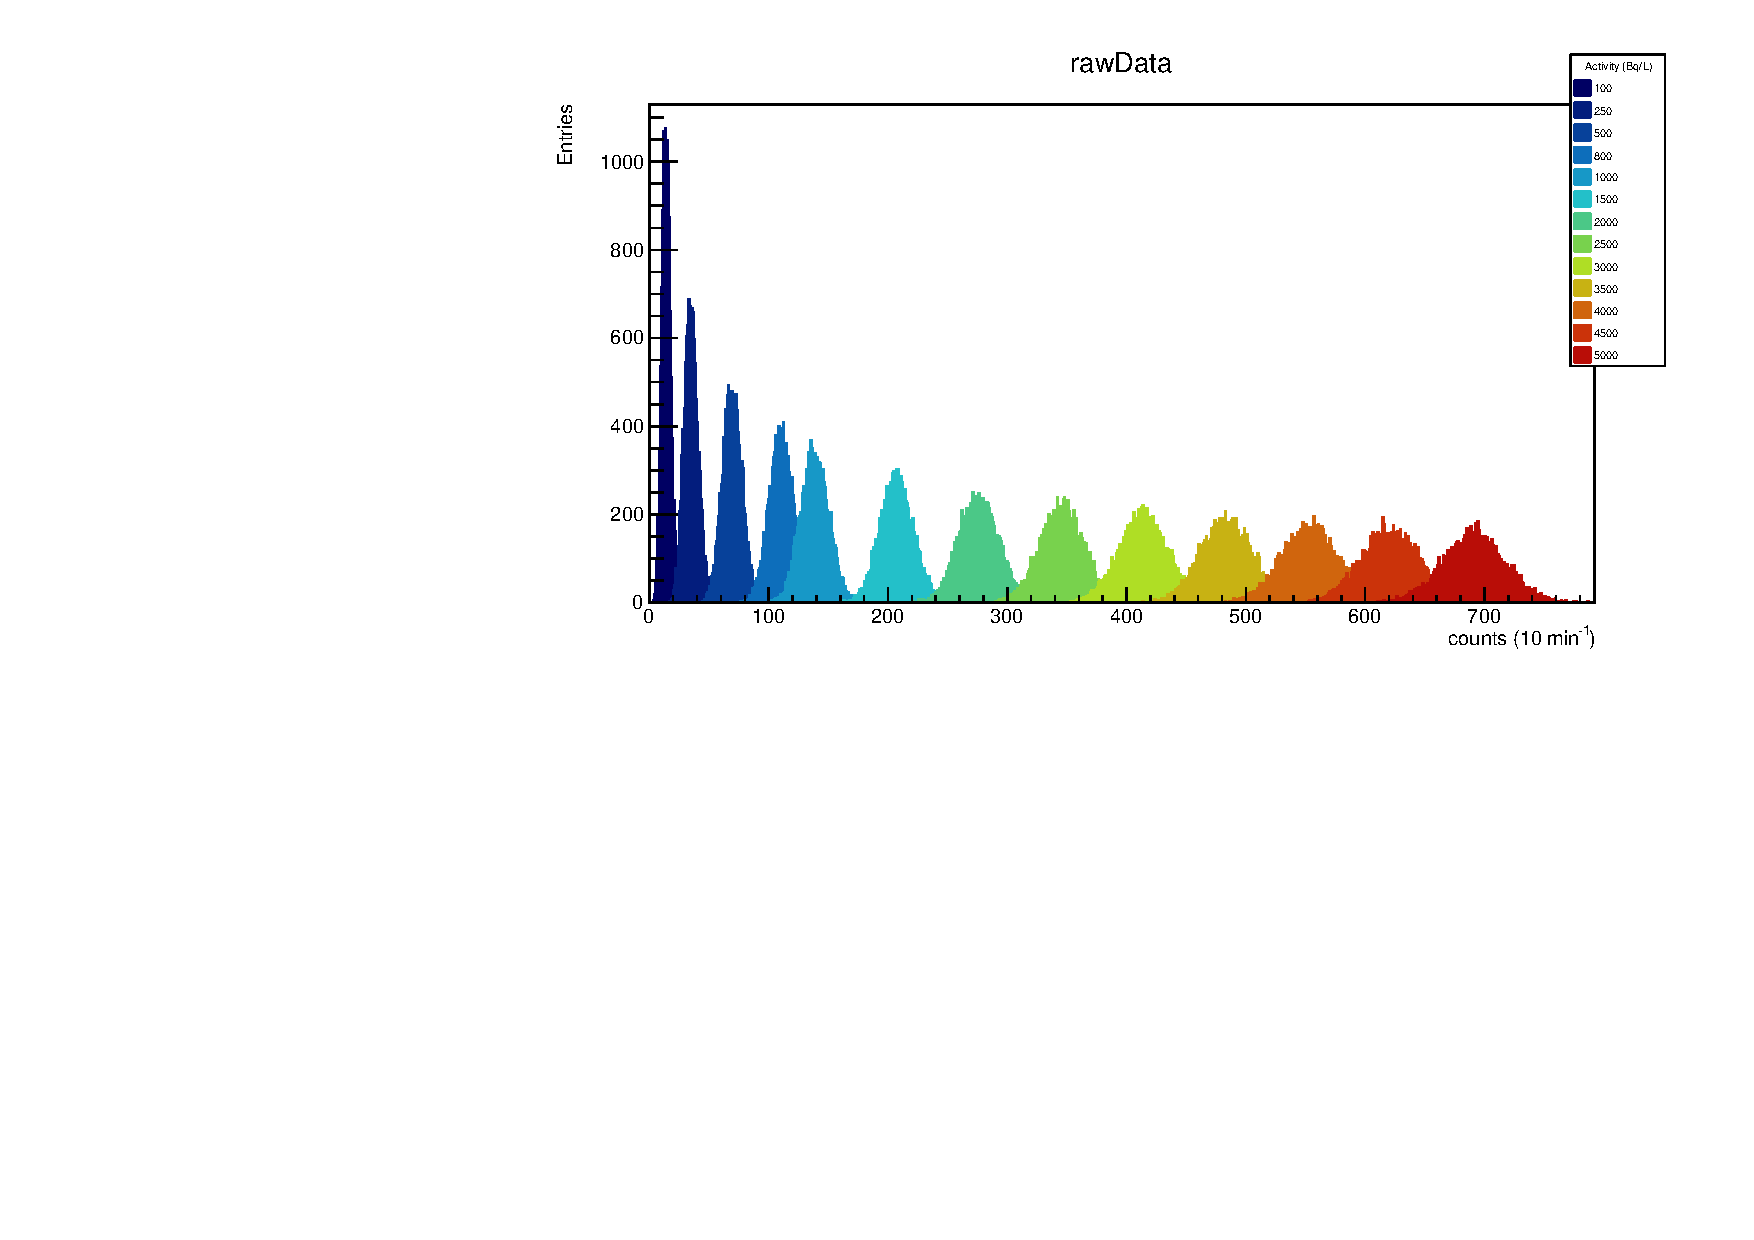
\includegraphics[width=\textwidth]{8SimulationsResults/82TRITIUMMonitor/821TRITIUMIFIC2/Dist_5Det_10min_250BqL.pdf}  
    \caption{\label{subfig:5Det10min250BqLSD}}
    \end{subfigure}
    \hfill
    \begin{subfigure}[b]{0.6\textwidth}
    \centering
    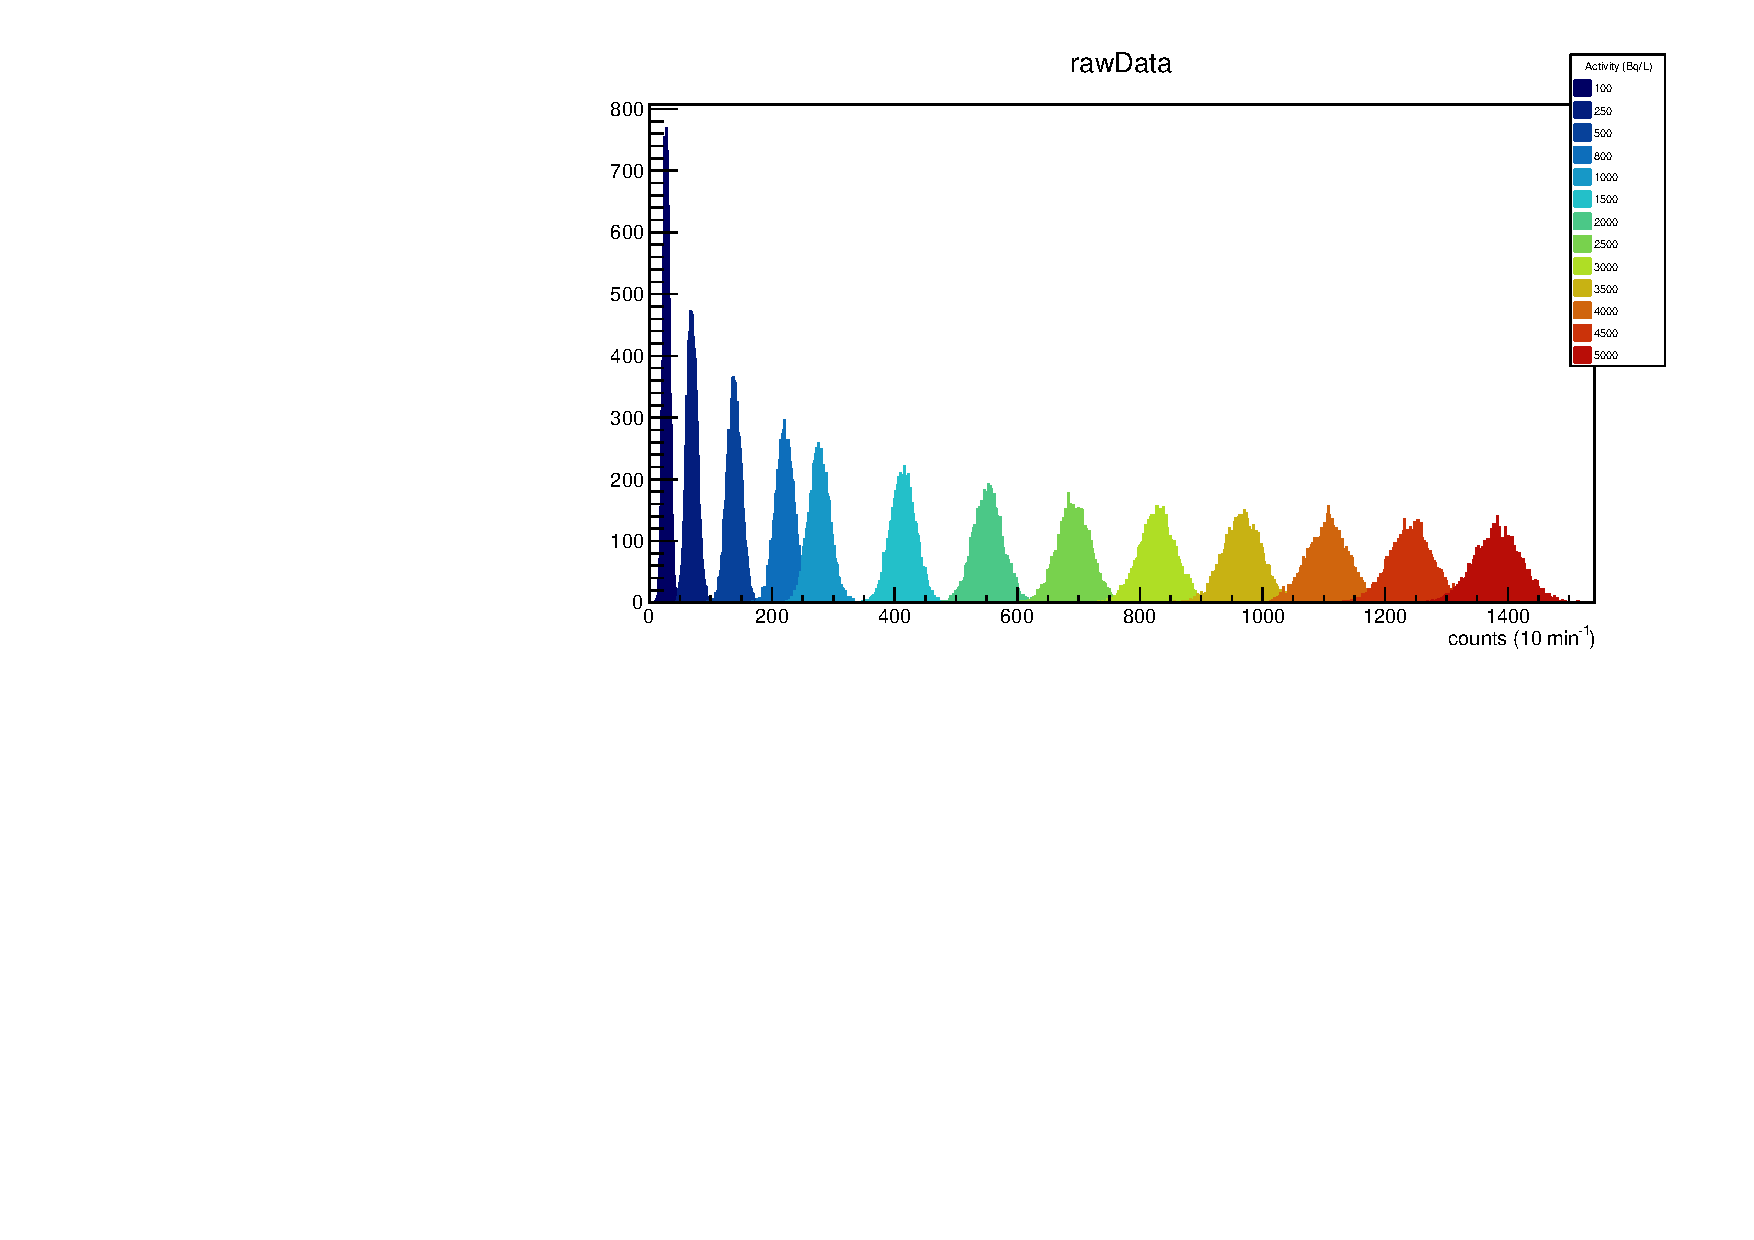
\includegraphics[width=\textwidth]{8SimulationsResults/82TRITIUMMonitor/821TRITIUMIFIC2/Dist_10Det_10min_250BqL.pdf}  
    \caption{\label{subfig:10Det10min250BqLSD}}
    \end{subfigure}
 \caption{The distribution of the tritium counts detected with several simulated TRITIUM-IFIC 2 prototypes a) 1, b) 5 and c) 10 for an integration counting time of $10~\min$.}
 \label{fig:SeveralDet250BqL10min}
\end{figure}

Again the reduction of the distribution width is clearly visible in these figures, improving the activity resolution of the detector. In this case, differences of $250~\becquerel/\liter$ are clearly distinguised using a integration counting time of $10~\min$ and measuring with 5 TRITIUM-IFIC 2 prototypes. 

The effect on the resolution, defined as the equation \ref{eq:Resolution}, is also studied as a function of both TRITIUM monitor characteristics, integration counting time and number of used prototypes, and shown in Figure \ref{fig:Resolution}.

\begin{equation}
\text{Resolution(\%)}=\frac{\text{FWHM}}{\text{centroid}}\cdot{}100
\label{eq:Resolution}
\end{equation}

\begin{figure}
\centering
    \begin{subfigure}[b]{0.45\textwidth}
    \centering
    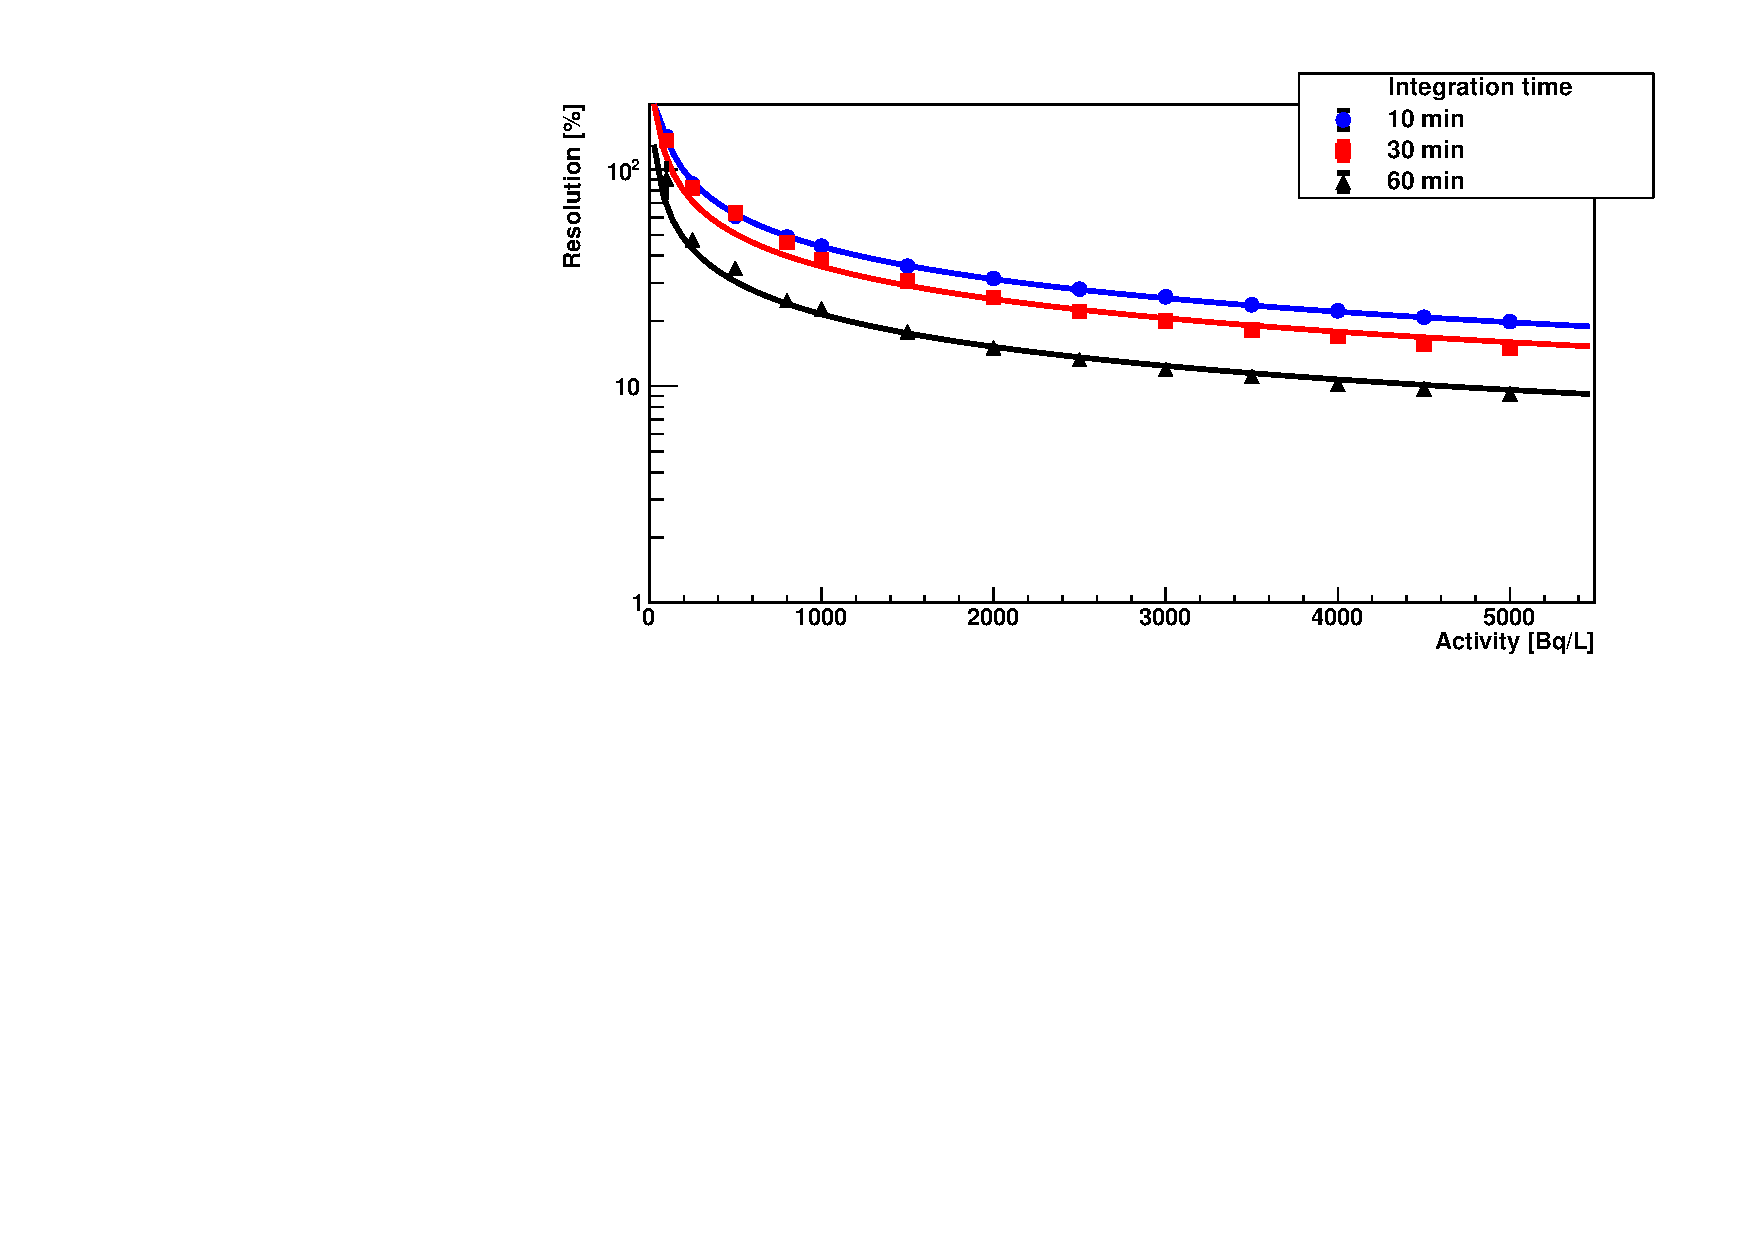
\includegraphics[width=\textwidth]{8SimulationsResults/82TRITIUMMonitor/821TRITIUMIFIC2/Results_Several_Times.pdf}  
    \caption{\label{subfig:ResolutionvsIntegrationCoutingTime}}
    \end{subfigure}
    \hfill
    \begin{subfigure}[b]{0.45\textwidth}
    \centering
    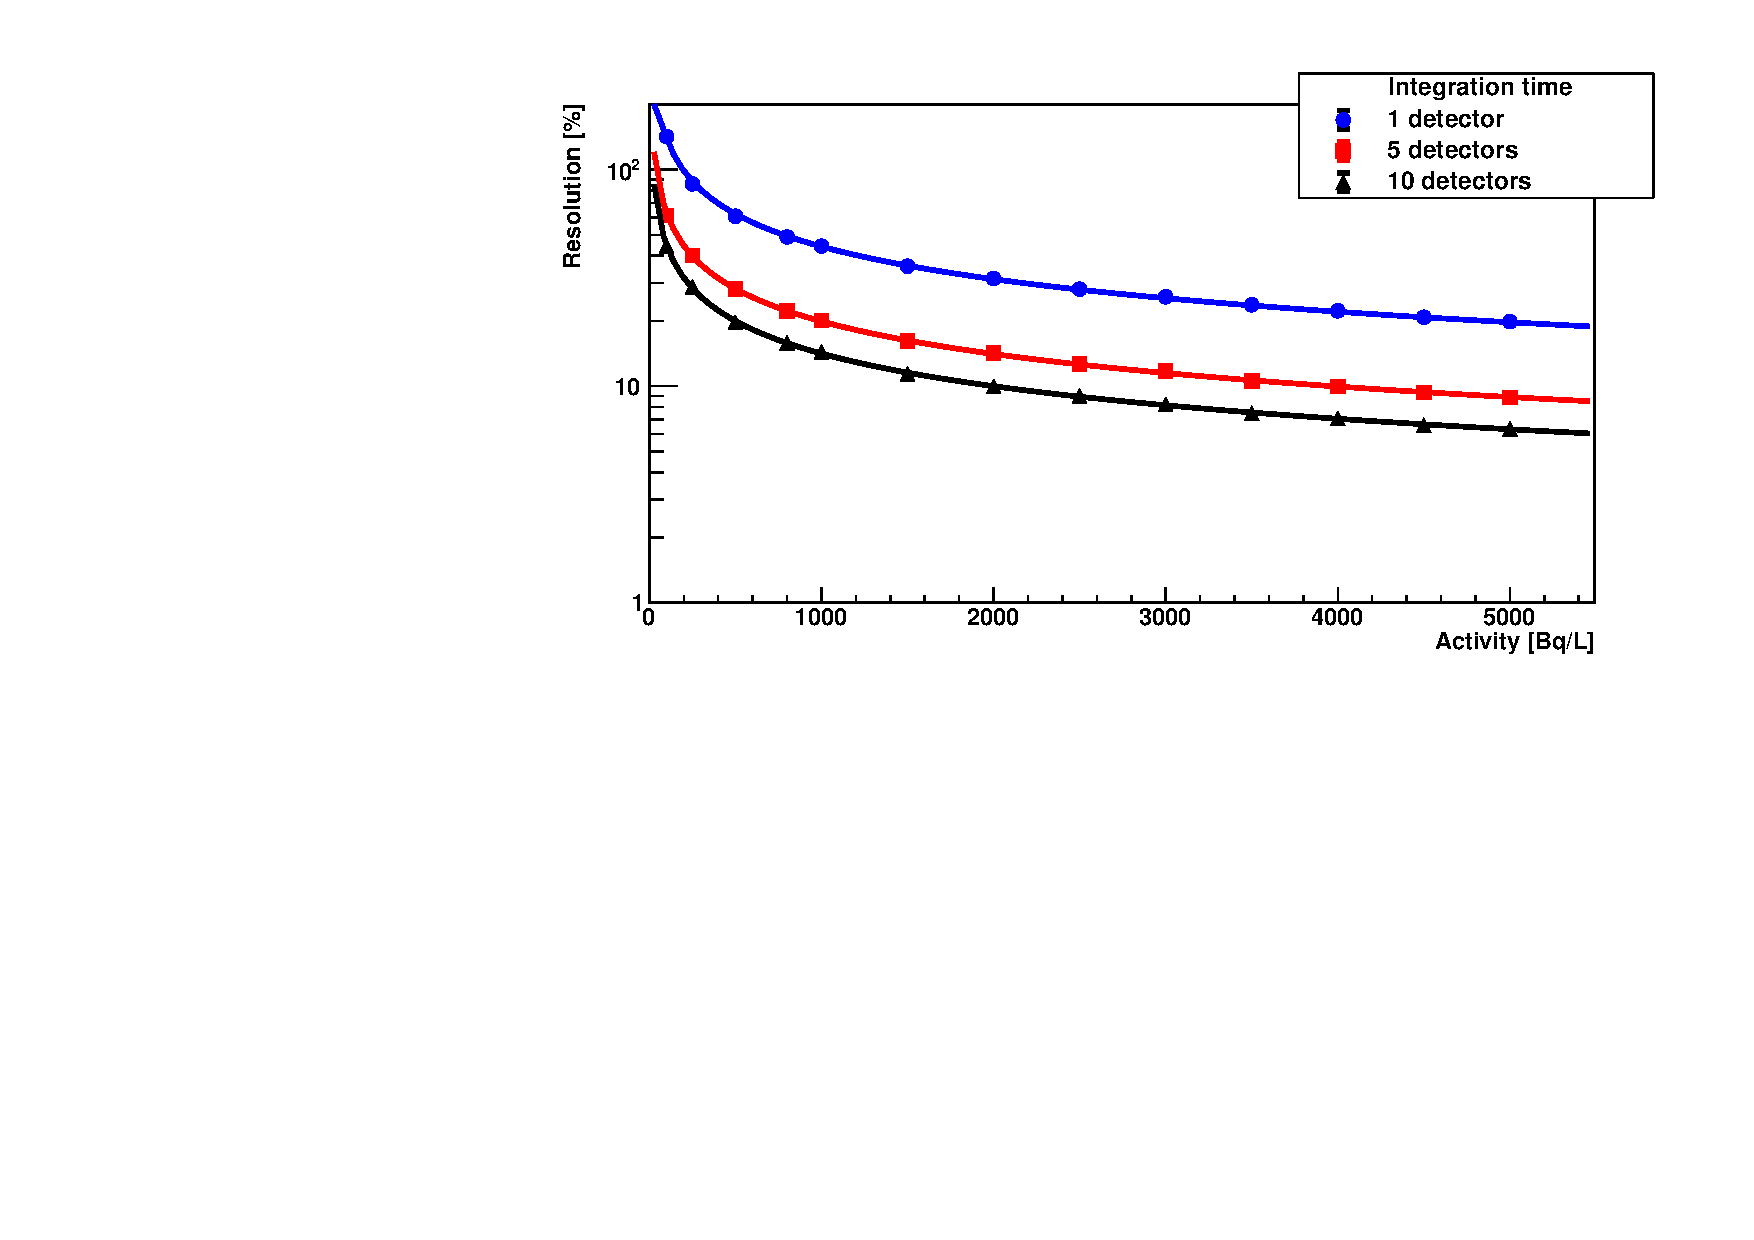
\includegraphics[width=\textwidth]{8SimulationsResults/82TRITIUMMonitor/821TRITIUMIFIC2/Results_Several_Detectors.pdf}  
    \caption{\label{subfig:ResolutionvsNumberDetectors}}
    \end{subfigure}
 \caption{Resolution of the TRITIUM-IFIC 2 prototype as a function of the a) integration counting time b) number of prototypes.}
 \label{fig:Resolution}
\end{figure}

A growing improvement can be observed in both cases and, as can be verified with the lines in the figure, the resolution of both cases fit to the expected behavior of the inverse of the root of accounts.

Therefore, both characteristics must be balanced based on the requirements and financial budget of the experiment. The activity difference, the distribution peaks of which are clearly distinguised for each different case of integration counting time and number of detectors used, is summarized in Table \ref{tab:DifferentCasesOfTI2}.

\begin{table}[htbp]
\centering{}%
\begin{tabular}{lccc}
\toprule 
\# of Detectors & $10~\min$ & $30~\min$ & $60~\min$ \tabularnewline
\midrule
\midrule 
1 & $<1000~\becquerel/\liter$ & $500~\becquerel/\liter$ & $200~\becquerel/\liter$ \tabularnewline
5 & $200~\becquerel/\liter$ & $150~\becquerel/\liter$ & $100~\becquerel/\liter$ \tabularnewline
10 & $150~\becquerel/\liter$ & $100~\becquerel/\liter$ & $\approx 50~\becquerel/\liter$ \tabularnewline
\bottomrule
\end{tabular}
\caption{Difference in activity that can be clearly distinguished for various cases of the TRITIUM-IFIC 2 prototype based on different integration counting times and different number of prototypes.}
\label{tab:DifferentCasesOfTI2}
\end{table}

The decision made in the TRITIUM experiment is to install 3 different TRITIUM-IFIC 2 prototypes, with which differences of $250~\becquerel/\liter$ are expected to be distinguished using an integration counting time of $30~\min$. These prototypes are expected to be installed  in Arrocampo dam as soon as possible. Two other TRITIUM-Aveiro 0 prototypes are being built and will be installed soon, along the one currently installed.

%Se ha realizado un ajuste lineal del centroide de las gaussianas de los ajustes (y su anchura como error) frente a la actividad usada. El rango utilizado en este caso ha sido mucho mayor debido a

%Tritium detection was studied using only one TRITIUM-IFIC 2 prototype, throguh the simulation of various activities of tritiated water. The integration count time used was $10~\min$ and continuous use of the detector during 3 months was simulated for each activity studied.


%PEORES RESULTADOS SIMULADOS QUE CON AVEIRO PERO MEJORES EXPERIMENTALMENTE. La diferencia debe de estar en que uno usa fibras pulida y limpiadas y el otro no.

%PREPARAR EN BACK UP EN LA PRESENTACIÓN EL CASO PARA 3 DETECTORES, YA QUE SERÁ NUESTRO CASO.
